\chapter{Analiza wymagań projektowych}
\section{Opis działania systemu}
\subsection{Cel i przeznaczenie systemu}
Celem systemu jest zwiększenie komfortu i~immersji podczas czytania
książek poprzez automatyczny dobór muzyki odtwarzanej w~tle. Muzyka
dobierana jest na podstawie emocji zawartych w
fragmencie tekstu, dzięki czemu użytkownik nie musi samodzielnie
wyszukiwać ani zmieniać utworów w~trakcie lektury.

\begin{figure}[htbp]
      \center
      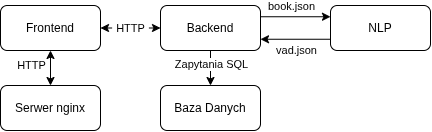
\includegraphics[width=0.7\linewidth]{figures/5/diagram_5.png}
      \caption{Uproszczony diagram architektury aplikacji}
      \label{fig:app_diagram}
\end{figure}

\subsection{Użytkownicy i role}
W~systemie wyróżniono dwie role użytkowników:
\begin{itemize}
    \item \textbf{Czytelnik:} główny użytkownik systemu. Dodaje książki
          do swojej biblioteki, czyta je w~aplikacji oraz słucha muzyki
          dobieranej automatycznie do czytanego fragmentu.
    \item \textbf{Administrator:} odpowiada za utrzymanie i~rozwój
          systemu. Zarządza biblioteką utworów muzycznych, dodaje nowe
          nagrania oraz aktualizuje modele uczenia maszynowego
          wykorzystywane do rozpoznawania emocji w~tekście.
\end{itemize}

\subsection{Główne funkcje}
System udostępnia następujące funkcje:
\begin{itemize}
    \item wgranie książki w~formacie EPUB do biblioteki użytkownika,
    \item automatyczna analiza emocjonalna całej książki po jej wgraniu,
          wykonywana i~zapisywana wraz z~położeniem fragmentów w~tekście,
    \item czytanie książki w~oknie przeglądarki internetowej wraz
          z~nawigacją po rozdziałach
    \item automatyczny dobór utworu muzycznego odpowiadającego nastrojowi
          aktualnie czytanego fragmentu
    \item odtwarzanie muzyki z~płynnymi przejściami między utworami,
    \item sterowanie odtwarzaniem: pominięcie utworu, pauza oraz regulacja
          głośności
    \item zarządzanie katalogiem utworów i~modelami uczenia maszynowego
          przez Administratora.
\end{itemize}
W~obecnej wersji system obsługuje książki w~języku angielskim w formacie epub ze strony
Standard E-books\cite{StandardEbooks}

\subsection{Główne komponenty i~ich współpraca}
\begin{itemize}
    \item \textbf{Frontend (React):} wyświetla książkę,
          śledzi aktualną pozycję czytania i~przekazuje ją do backendu,
          obsługuje odtwarzacz audio oraz sterowanie muzyką.
    \item \textbf{Backend (FastAPI):} przyjmuje wgrane książki, dzieli je
          na zdania i~uruchamia ich analizę w~tle. Podczas czytania
          dobiera utwór na podstawie pozycji w~książce i~zwraca
          frontendowi jego identyfikator. Nie przesyła plików audio.
    \item \textbf{Moduł NLP (DeBERTa-v3-base):} zamienia zdania na wartości
          nastroju w~modelu VAD.
    \item \textbf{Baza danych (SQLite):} przechowuje zdania książek wraz
          z~wartościami VAD oraz katalog utworów z~metadanymi nastroju.
    \item \textbf{Serwer plików (Nginx):} udostępnia pliki audio
          bezpośrednio przeglądarce.
\end{itemize}



\section{Wymagania funkcjonalne i niefunkcjonalne}
\subsection{Wymagania funkcjonalne}
\begin{itemize}
      \item[\textbf{FU1:}] Użytkownik ma możliwość wgrania pliku książki w formacie \textit{.epub}.
      \item[\textbf{FU2:}] Aplikacja prezentuje listę wgranych książek wraz ze statusem ich przetwarzania.
      \item[\textbf{FU3:}] Aplikacja umożliwia odczyt treści książki z automatycznym stronicowaniem oraz
      nawigacją po rozdziałach (spis treści).
      \item[\textbf{FU4:}] Aplikacja automatycznie dobiera i odtwarza podkład muzyczny na podstawie nastroju
      (emocji) aktualnie czytanego fragmentu tekstu.
      \item[\textbf{FU5:}] Aplikacja umożliwia kontrolę odtwarzacza audio (wstrzymanie, wznowienie, regulacja
      głośności oraz pominięcie utworu na kolejny z tej samej kategorii nastroju).
      \item[\textbf{FU6:}] Aplikacja prezentuje użytkownikowi informację o aktualnie rozpoznanym nastroju tekstu
      oraz tytule/identyfikatorze odtwarzanego utworu.
      \item[\textbf{FU7:}] Użytkownik ma możliwość usunięcia wybranej książki z biblioteki.
\end{itemize}

\subsection{Wymagania niefunkcjonalne}
\begin{itemize}
      \item[\textbf{NF1:}] \textbf{Asynchroniczność przetwarzania:} Parsowanie plików EPUB oraz inferencja modelu
      NLP muszą odbywać się w tle (asynchronicznie), nie blokując responsywności interfejsu użytkownika.

      \item[\textbf{NF2:}] \textbf{Płynność przejść audio (crossfading):} Zmiana odtwarzanego utworu lub zmiana
      kategorii nastroju w trakcie czytania musi odbywać się w sposób płynny (płynne wyciszanie poprzedniego i
      pogłaśnianie kolejnego utworu), bez gwałtownych przerw i trzasków dźwiękowych.

      \item[\textbf{NF3:}] \textbf{Responsywność i dynamiczne stronicowanie:} Algorytm podziału tekstu na strony
      w czytniku musi automatycznie dostosowywać liczbę i objętość stron do aktualnego rozmiaru okna przeglądarki
      (viewportu) i rozdzielczości ekranu.

      \item[\textbf{NF4:}] \textbf{Predykcja z wyprzedzeniem (lookahead):} W celu uniknięcia opóźnień w doborze
      ścieżki dźwiękowej, aplikacja powinna pobierać predykcje nastroju z wyprzedzeniem (dla bieżącej oraz
      kolejnych stron tekstu).

      \item[\textbf{NF5:}] \textbf{Konteneryzacja i łatwość wdrożenia:} Wszystkie komponenty systemu (frontend,
      backend, serwis NLP, serwer multimediów) muszą być skonteneryzowane (Docker) i umożliwiać uruchomienie
      całego środowiska za pomocą pojedynczego polecenia (\textit{docker compose up}).

      \item[\textbf{NF6:}] \textbf{Modularność architektury:} Usługa inferencji modelu uczenia maszynowego (NLP)
      musi stanowić niezależną usługę od głównego serwera aplikacji, komunikującą się za pośrednictwem protokołu
      HTTP/REST API.

      \item[\textbf{NF7:}] \textbf{Zarządzanie przestrzenią dyskową:} System powinien okresowo usuwać pliki
      sesyjne oraz przetworzone dane starsze niż określony czas retencji, zapobiegając nadmiernemu zużyciu
      pamięci masowej serwera.
\end{itemize}



\section{Przypadki użycia}
\subsection{Spis przypadków użycia}
\begin{itemize}
      \item[\textbf{PU1:}] Wgranie pliku \textit{.epub} książki i uruchomienie wstępnego procesu.
      \item[\textbf{PU2:}] Przeglądanie biblioteki wgranych książek i monitorowanie stanu
      procesowania.
      \item[\textbf{PU3:}] Usunięcie książki z biblioteki przez użytkownika. 
      \item[\textbf{PU4:}] Otwarcie i lektura książki w specjalnym oknie.
      \item[\textbf{PU5:}] Nawigacja po stronach za pomocą odopwiednich przycisków lub menu po 
      rozdziałach
      \item[\textbf{PU6:}] Automatyczne odtwarzanie i zmiana utworów w tle w
      oparciu o wykryty nastrój czytanej treści.
      \item[\textbf{PU7:}] Manualna regulacja głośności, wstrzymywanie odtwarzania
        oraz pomijanie utworów.
\end{itemize}

\subsection{Opis wybranych przypadków użycia}
\subsubsection{PU1: Wgranie pliku i procesowanie.}
\begin{enumerate}
      \item Użytkownik wybiera opcję wgrania pliku (\textit{Upload epub}) i wskazuje plik z dysku 
      lokalnego.
      \item System weryfikuje poprawność formatu wskazanego pliku (wymagany format \textit{.epub}).
      \item Po pomyślnej walidacji książka zostaje dodana do biblioteki ze statusem informującym o 
      rozpoczęciu przetwarzania.
      \item System dokonuje asynchronicznej analizy struktury książki oraz wyznaczenia profilu 
      emocjonalnego tekstu.
      \item Po zakończeniu procesu status książki zostaje zaktualizowany na ukończony (\textit{done}),
      umożliwiając użytkownikowi jej odczyt.
\end{enumerate}

\subsubsection{PU6: Automatyczne odtwarzanie muzyki.}
\begin{enumerate}
      \item Po otworzeniu książki do czytania, do warstwy serwerowej wysyłane są indeksy aktualnych
      oraz przyszłych zdań.
      \item Aplikacja serwerowa analizuje dane zdania i porównuje je  z wygenerowaymi wcześniej
      wartościami emocji dla danego tekstu.
      \item Warstwa serwerowa zwraca etykietę emocji oraz jej tzw. pewność, na podstawie, której
      dobierany jest utwór w warstwie prezentacji.
      \item Warstwa prezentacji dobiera utwór oraz odtwarza go ze statycznego serwera.
\end{enumerate}

\begin{figure}[htbp]
      \center
      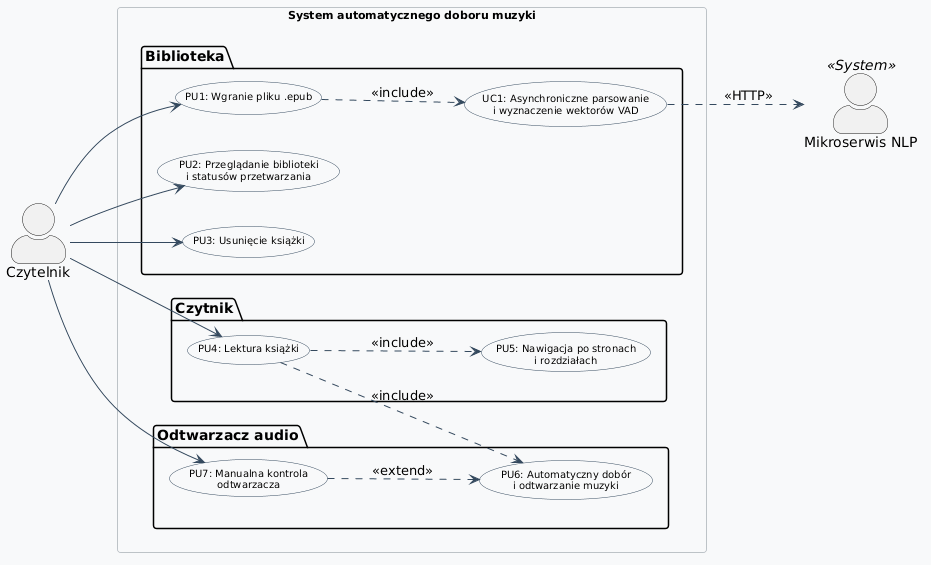
\includegraphics[width=0.9\linewidth]{figures/5/diagram_pu.png}
      \caption{Diagram przypadków użycia}
      \label{fig:usecase_diagram}
\end{figure}



\section{Projekt interfejsu REST/API}
\subsection{Punkty dostępu udostępniane przez aplikację}
\begin{table}[htbp]
      \center
      \caption{Tablica punktów końcowych aplikacji}
      \label{tab:endpoints}
      \begin{tabular}{l l p{7cm}}
          \toprule
          Metoda & Ścieżka & Opis \\
          \midrule
          POST   & \textit{/session/init}            & Inicjalizacja sesji
          użytkownika i nadanie ciasteczka sesyjnego (\textit{sid}) \\
          POST   & \textit{/books/upload\_epub}      & Przesłanie pliku EPUB
          i uruchomienie asynchronicznego przetwarzania \\
          GET    & \textit{/books/mine}              & Pobranie listy książek
          przypisanych do bieżącej sesji użytkownika \\
          GET    & \textit{/books/\{job\_id\}/status}  & Pobranie aktualnego
          statusu przetwarzania książki \\
          GET    & \textit{/books/\{job\_id\}/content} & Pobranie
          przetworzonej treści książki w formacie JSON \\
          DELETE & \textit{/books/\{job\_id\}}        & Usunięcie książki
          oraz powiązanych plików z serwera \\
          POST   & \textit{/predictions/\{job\_id\}}  & Klasyfikacja
          nastroju/emocji dla wskazanego fragmentu zdań \\
          GET    & \textit{/health}                  & Sprawdzenie stanu
          dostępności serwisu (health check) \\
          \midrule[\heavyrulewidth]
          \multicolumn{3}{l}{\textit{Wewnętrzny mikroserwis NLP (komunikacja
          międzykontenerowa):}} \\
          \midrule
          POST   & \textit{/prediction/\{job\_id\}}   & Wyznaczenie wektorów 
          VAD dla zdań książki przez model DeBERTa \\
          \bottomrule

      \end{tabular}
\end{table}




\FloatBarrier
\subsection{Struktura ciała wybranych zapytań i generowanych plików}
Ciała zapytań podczas komunikacji są oparte na strukturze plików \textit{.json}. Poniżej podane
zostały przykłady budowy takich zapytań.
\subsubsection{Budowa pliku \textit{book.json} (przeprocesowanej książki z formatu \textit{.epub})}
\begin{lstlisting}[style=jsonStyle, caption={
            Przykład przeprocesowanej książki, tutaj: \textit{"At the Mountains of Madness"},
            Autorstwa \textit{H. P. Lovecraft'a}\cite{MountainOfMadnessLovecrafr}
}, label={lst:json_processed}]
{
  "metadata": {
    "title": "At the Mountains of Madness",
    "author": "H. P. Lovecraft",
    "source_format": "standard_ebooks",
    "sentence_splitter": "pysbd 0.3.4",
    "created_at": "2026-11-13T12:36:26",
    "num_chapters": 12,
    "num_sentences": 1352
  },
  "chapters": [
    {
      "chapter_id": 1,
      "title": "I",
      "paragraphs": [
        {
          "paragraph_id": 1,
          "sentences": [
            {
              "id": 1,
              "text": "I am forced into speech because men of science have refused to follow my advice without knowing why."
            },
      ...
\end{lstlisting}

\subsubsection{Struktura pliku \textit{vad.json} (listy id z ich predykcjami)}
\begin{lstlisting}[style=jsonStyle, caption={
      Plik zawiera predykcje \textit{VAD} dla każdego id zdania, obliczone centroidy dla etykiet, 
      przesunięcie środka skali, oraz promień neutralności.
}, label{lst:json_vad}]
{
    "meta": {
        "model_name": "deberta-vad-seed42",
        "columns": [
            "valence",
            "arousal",
            "dominance"
        ],
        "config": {
            "centroids": {
                "joy": [
                    0.3801,
                    0.5073,
                    0.3842
                ],
                "sadness": [
                    -0.5985,
                    0.0093,
                    -0.5293
                ],
                "tense": [
                    -0.3327,
                    0.4785,
                    -0.0
                ],
                "calm": [
                    0.2694,
                    -0.2047,
                    -0.3125
                ]
            },
            "r_neutral": 0.1972,
            "k": [
                0.5272,
                0.4495,
                0.725
            ],
            "center": [
                -0.1261,
                0.1999,
                -0.0421
            ]
        }
    },
    "vad": {
        "1": [
            -0.4039,
            0.2931,
            -0.2142
        ],
      ...
\end{lstlisting}

\subsubsection{Zapytanie i odpowiedź serwera zawierający etykietę emocji}
\begin{lstlisting}[style=jsonStyle, caption={
      Zapytanie i odpowiedź serwera na zapytanie \textit{/predictions/{job\_id}}, przekazujące etykietę emocji
      pewność oraz różnice od drugiej najpewniejszej odpowiedzi
}, label={lst:predictions_answer}]
# Zapytanie
{
      "sentence_ids": [488, 489, 490, 491, 492, 493, ...]
}

# Odpowiedz
{
    "job_id": "37d9141d50e846c2bb4e5c9913c878e0",
    "label": "tense",
    "certainty": 0.6666666666666666,
    "margin": 0.4286
}
\end{lstlisting}

\subsubsection{Generowany plik \textit{manifest.json}, używany jako lista utworów dla warstwy 
prezentacji}
\begin{lstlisting}[style=jsonStyle, caption={
      Struktura pliku \textit{manifest.json}, generowanego przez serwer nginx z muzyką
}, label={lst:manifest}]
[
      {
            "filename": "01 - DREAMCATCHER by Onycs.mp3",
            "id": "01 - DREAMCATCHER by Onycs",
            "category": "calm",
            "path": "calm/01 - DREAMCATCHER by Onycs.mp3"
      },
      {
            "filename": "05 - Tension Rising.mp3",
            "id": "05 - Tension Rising",
            "category": "tense",
            "path": "tense/05 - Tension Rising.mp3"
      }
]
\end{lstlisting}

\section{Metoda połączenia modelu uczenia maszynowego z aplikacją}
Aplikacja łączy się z modelem poprzez sieć. Kontener zawierający obsługę modelu uczenia maszynowego
jak i całą logikę z nim związaną udostępnia \textit{endpoint}, który otrzymuje \textit{.json}
zawierający przeprocesowaną książke, a następnie zwraca nowy plik zawierający predykcje wartości
dla każdego ze zdań w książce oraz dodatkowe parametry. Taki sposób procesowania przyspiesza późniejsze predykcje kosztem
dłuższego oczekiwania wstępnego.
\begin{figure}[htbp]
      \center
      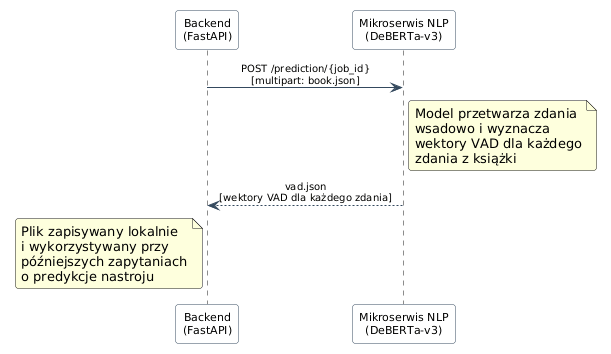
\includegraphics[width=0.7\linewidth]{figures/5/flowdiagram_55.png}
      \caption{Diagram przepływu dla połączenia modelu z warstwą serwerową}
      \label{fig:flow_diagram_nlp_backend}
\end{figure}


\section{Metoda powiązania warstwy prezentacji z serwerem na dane}
Warstwa prezentacji pobiera muzykę bezpośrednio ze statycznego serwera nginx. Aby mieć możliwość
odtwarzania kolejnego utworu z tego samego nastroju, serwer przy starcie generuje plik 
\textit{"manifest.json"} zawierający indeks utworów, serwowaną ścieżkę, oraz jego nastrój. Warstwa
prezentacji pobiera, ten plik przy uruchomieniu w przeglądarce, a następnie używa go do śledzenia
ostatnio odtwarzanych utworów. Dzięki takiemu rozwiązaniu obraz kontenera frontendu nie zawiera 
plików audio, muzyka przechowywana jest wyłącznie w wolumenie serwera nginx. Pozwala to na łatwe 
dodawanie i usuwanie utworów bez ponownego budowania i uruchamiania warstwy prezentacji.
\begin{figure}[htbp]
      \center
      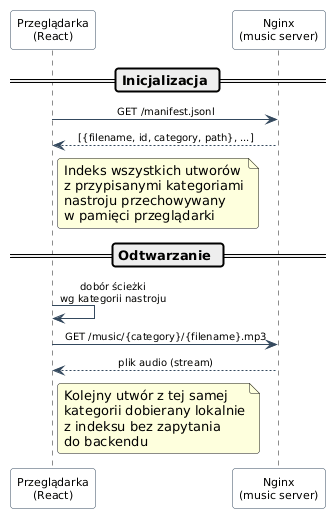
\includegraphics[width=0.6\linewidth]{figures/5/flow_56.png}
      \caption{Diagram przepływu pomiędzy warstwą prezentacji, a serwerem statycznym}
      \label{fig:flowdiagram_frontend_nginx}
\end{figure}



